\tikzset{every picture/.style={line width=0.75pt}} %set default line width to 0.75pt        

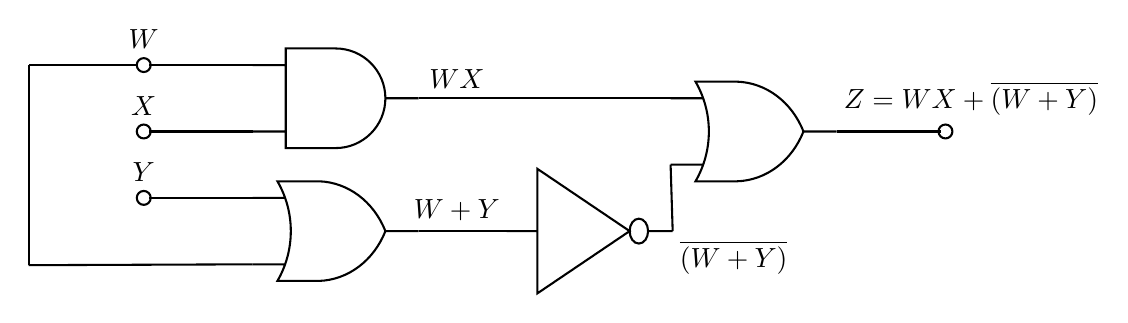
\begin{tikzpicture}[x=0.75pt,y=0.75pt,yscale=-1,xscale=1]
%uncomment if require: \path (0,393); %set diagram left start at 0, and has height of 393

%Straight Lines [id:da23815456210484298] 
\draw    (189.71,157) -- (139.64,157) ;
\draw [shift={(137.29,157)}, rotate = 180] [color={rgb, 255:red, 0; green, 0; blue, 0 }  ][line width=0.75]      (0, 0) circle [x radius= 3.35, y radius= 3.35]   ;
%Straight Lines [id:da04610179645106571] 
\draw    (189.71,189) -- (139.64,189) ;
\draw [shift={(137.29,189)}, rotate = 180] [color={rgb, 255:red, 0; green, 0; blue, 0 }  ][line width=0.75]      (0, 0) circle [x radius= 3.35, y radius= 3.35]   ;
%Shape: And Gate [id:dp1564557077664277] 
\draw   (205.71,149) -- (229.71,149) .. controls (242.96,149) and (253.71,159.75) .. (253.71,173) .. controls (253.71,186.25) and (242.96,197) .. (229.71,197) -- (205.71,197) -- (205.71,149) -- cycle (189.71,157) -- (205.71,157) (189.71,189) -- (205.71,189) (253.71,173) -- (269.71,173) ;
%Straight Lines [id:da4661863224212748] 
\draw    (391.13,173) -- (280,173) -- (269.71,173) ;
%Straight Lines [id:da6073723811431462] 
\draw    (189.71,221) -- (139.64,221) ;
\draw [shift={(137.29,221)}, rotate = 180] [color={rgb, 255:red, 0; green, 0; blue, 0 }  ][line width=0.75]      (0, 0) circle [x radius= 3.35, y radius= 3.35]   ;
%Shape: Or Gate [id:dp34982237474249467] 
\draw   (201.71,213) -- (221.71,213) .. controls (235.66,213.43) and (248.13,222.78) .. (253.71,237) .. controls (248.13,251.22) and (235.66,260.57) .. (221.71,261) -- (201.71,261) .. controls (210.29,246.15) and (210.29,227.85) .. (201.71,213) -- cycle (189.71,221) -- (205.71,221) (189.71,253) -- (205.71,253) (253.71,237) -- (269.71,237) ;
%Straight Lines [id:da4284855074469899] 
\draw    (134.29,157) -- (81.87,157) ;
%Straight Lines [id:da5958317835136014] 
\draw    (81.87,253.42) -- (81.87,157) ;
%Straight Lines [id:da993377758021355] 
\draw    (81.87,253.42) -- (189.71,253) ;
%Straight Lines [id:da05592416301039271] 
\draw    (312.13,237) -- (269.71,237) ;
%Shape: Not/Inverter Gate [id:dp7110148584625413] 
\draw   (326.95,207) -- (371.39,237) -- (326.95,267) -- (326.95,207) -- cycle (312.13,237) -- (326.95,237) (380.28,237) -- (392.13,237) (371.39,237) .. controls (371.39,233.69) and (373.38,231) .. (375.84,231) .. controls (378.29,231) and (380.28,233.69) .. (380.28,237) .. controls (380.28,240.31) and (378.29,243) .. (375.84,243) .. controls (373.38,243) and (371.39,240.31) .. (371.39,237) -- cycle ;
%Shape: Or Gate [id:dp6675241851427653] 
\draw   (403.13,165) -- (423.13,165) .. controls (437.08,165.43) and (449.55,174.78) .. (455.13,189) .. controls (449.55,203.22) and (437.08,212.57) .. (423.13,213) -- (403.13,213) .. controls (411.71,198.15) and (411.71,179.85) .. (403.13,165) -- cycle (391.13,173) -- (407.13,173) (391.13,205) -- (407.13,205) (455.13,189) -- (471.13,189) ;
%Straight Lines [id:da5356554710077354] 
\draw    (392.13,237) -- (391.13,205) ;
%Straight Lines [id:da3264629812941331] 
\draw    (471.13,189) -- (521.2,189) ;
\draw [shift={(523.55,189)}, rotate = 0] [color={rgb, 255:red, 0; green, 0; blue, 0 }  ][line width=0.75]      (0, 0) circle [x radius= 3.35, y radius= 3.35]   ;

% Text Node
\draw (137.29,150.6) node [anchor=south] [inner sep=0.75pt]    {$W$};
% Text Node
\draw (137.29,182.6) node [anchor=south] [inner sep=0.75pt]    {$X$};
% Text Node
\draw (288.13,169.6) node [anchor=south] [inner sep=0.75pt]    {$WX$};
% Text Node
\draw (137.29,214.6) node [anchor=south] [inner sep=0.75pt]    {$Y$};
% Text Node
\draw (288.13,233.6) node [anchor=south] [inner sep=0.75pt]    {$W+Y$};
% Text Node
\draw (394.13,240.4) node [anchor=north west][inner sep=0.75pt]    {$\overline{( W+Y)}$};
% Text Node
\draw (473.13,182.6) node [anchor=south west] [inner sep=0.75pt]    {$Z=WX+\overline{( W+Y)}$};


\end{tikzpicture}
